\chapter{Pyhop}

Para resolver un problema tenemos tres fases
\begin{enumerate}
   \item Modelato
   \item Planificación
   \item Ejecución
\end{enumerate}

El problema se define como una declaración de un nuevo estado del mundo (inicial), y una declaración de un objetivo.
El \textbf{dominio}, son las acciones disponibles, que se estructuran en dos niveles: tareas/operadores y métodos.


\begin{itemize}
	\item Información estática: no cambia durante la ejecución del
problema y que sirve de soporte. Por ejemplo: distancias
entre ciudades.
	\item Información dinámica: representa el estado actual del
mundo. Por ejemplo: cantidad de dinero disponible por el
agente en un momento determinado
\end{itemize}

\begin{figure}[htbp]
   \centering
   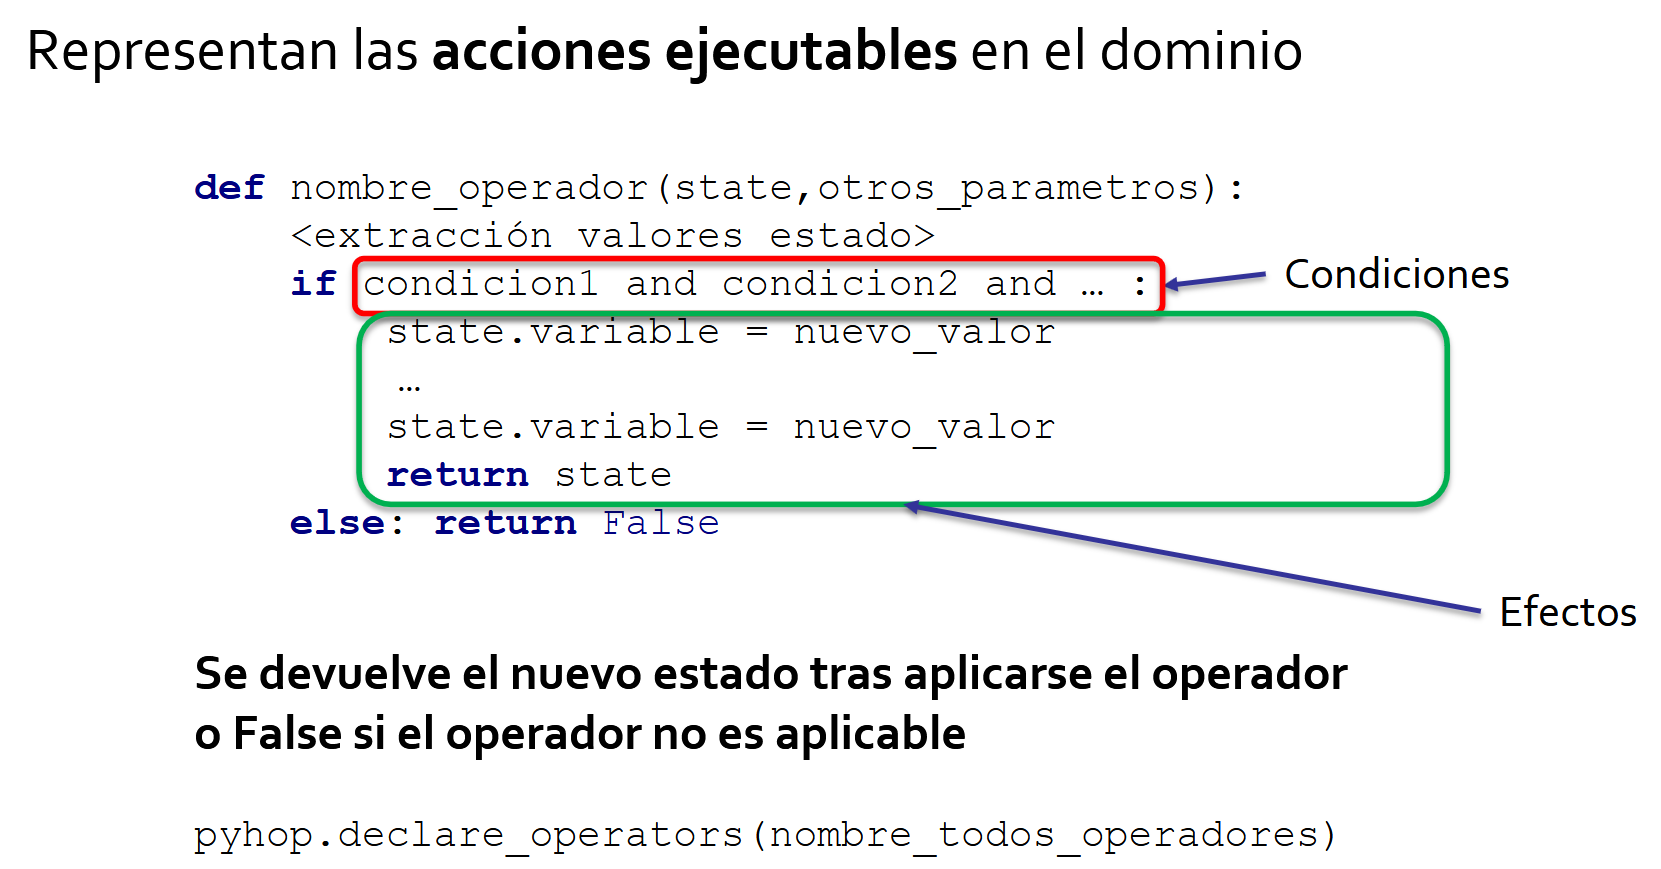
\includegraphics{images/03/operador.png}
   \caption{Como definir un operador en Pyhop}
   \label{fig:03/operador}
\end{figure}

% // TODO faltan ejemplos de Pyhop pero no pasa nada.

Los elementos básicos de \texttt{pyhop} son:
\begin{itemize}
   \item \textbf{Estado}: es un diccionario que representa el estado del mundo.
   \item \textbf{Tareas}: son tareas que identifican un objetivo (estado final) que se quiere alcanzar. 
   Las tareas primitivas son aquellas que se pueden ejecutar directamente y resolver con operadores, y las tareas compuestas son aquellas que se descomponen en otras tareas o acciones.
   \item \textbf{Operadores}: son funciones que toman un estado y devuelven un nuevo estado. \ul{\textbf{No} se pueden descomponer.}
   \item \textbf{Métodos}: representan una forma distinta de resolver una tarea. Están formados por un conjunto de tareas y operadores (acciones) que hay que ejecutar y/o alcanzar en un orden establecido para lograr resolver la tarea de nivel superior.\\
   Estas tareas y operadores se organizan de forma secuencial
\end{itemize}